\subsubsection{Handler}
The \textbf{Handler} layer manages the requests it receives from AWS\textsubscript{G} API Gateway and calls the other layers to fulfill them.\\
It is divided in domains and every domain contains a number of AWS\textsubscript{G} Lambda functions, the effective handlers of the requests. Finally, every function is located in file of its own.\\
To represent this, we will use the following package diagram, where every file/function is a unit inside the specific package.

\begin{figure}[H]
\centering
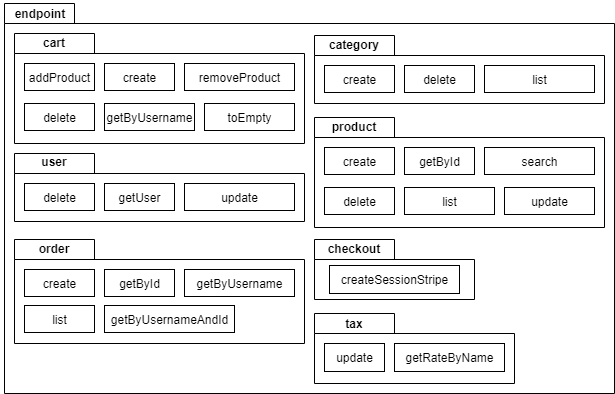
\includegraphics[scale=0.65]{res/Architettura/Backend/img/handler_package}\\
\caption{Back-end\textsubscript{G} Handler layer package diagram}
\end{figure}

Through this sequence diagram, we will show how a request can be fulfilled by all the layers. In this example, we represent the process of obtaining the details of a product and sending them to the front-end\textsubscript{G}.

\begin{figure}[H]
\centering
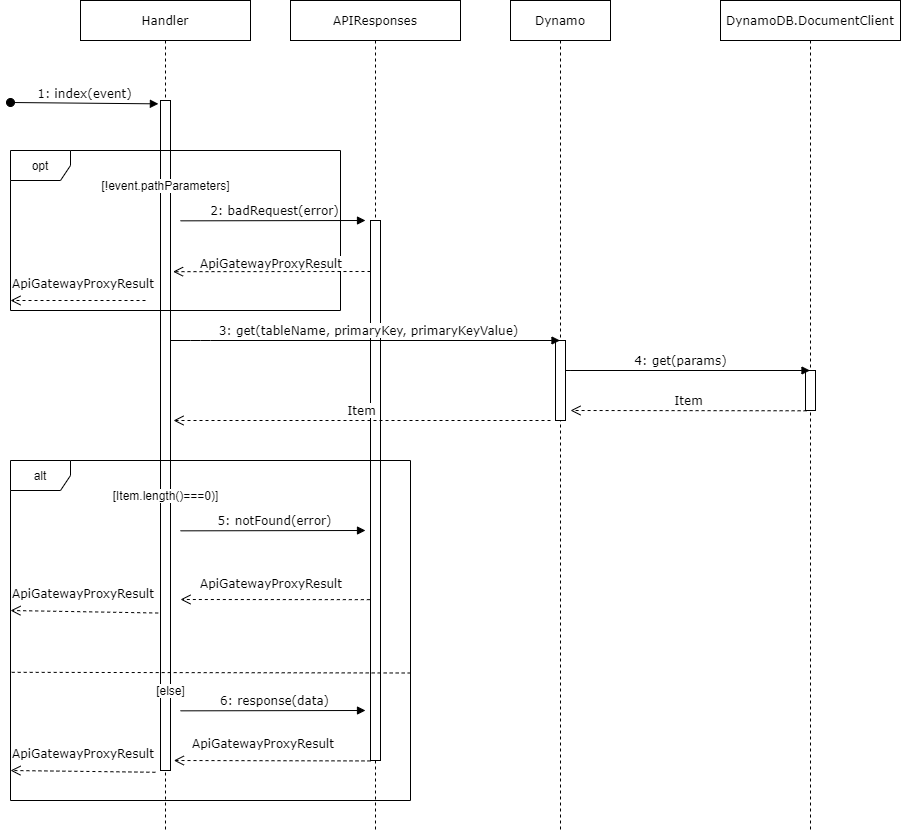
\includegraphics[scale=0.45]{res/Architettura/Backend/img/diagrammaSequenzaRicezioneProdotto}\\
\caption{Back-end\textsubscript{G} sequence diagram: obtaining product details}
\end{figure}

\begin{itemize}
\item \textbf{Handler} is how the function is called inside the \textit{getById} file, inside the \textit{product} domain;
\item \textbf{APIResponses} is a module containing functions inside the \textit{lib} package and manages the response to the front-end\textsubscript{G};
\item \textbf{Dynamo} is the dynamo module inside the \textit{service} module;
\item \textbf{DynamoDB.DocumentClient} is a class of the \textit{AWS-sdk} library that represents the effective database.

\end{itemize}



